% Options for packages loaded elsewhere
\PassOptionsToPackage{unicode}{hyperref}
\PassOptionsToPackage{hyphens}{url}
%
\documentclass[
]{article}
\usepackage{amsmath,amssymb}
\usepackage{lmodern}
\usepackage{ifxetex,ifluatex}
\ifnum 0\ifxetex 1\fi\ifluatex 1\fi=0 % if pdftex
  \usepackage[T1]{fontenc}
  \usepackage[utf8]{inputenc}
  \usepackage{textcomp} % provide euro and other symbols
\else % if luatex or xetex
  \usepackage{unicode-math}
  \defaultfontfeatures{Scale=MatchLowercase}
  \defaultfontfeatures[\rmfamily]{Ligatures=TeX,Scale=1}
\fi
% Use upquote if available, for straight quotes in verbatim environments
\IfFileExists{upquote.sty}{\usepackage{upquote}}{}
\IfFileExists{microtype.sty}{% use microtype if available
  \usepackage[]{microtype}
  \UseMicrotypeSet[protrusion]{basicmath} % disable protrusion for tt fonts
}{}
\makeatletter
\@ifundefined{KOMAClassName}{% if non-KOMA class
  \IfFileExists{parskip.sty}{%
    \usepackage{parskip}
  }{% else
    \setlength{\parindent}{0pt}
    \setlength{\parskip}{6pt plus 2pt minus 1pt}}
}{% if KOMA class
  \KOMAoptions{parskip=half}}
\makeatother
\usepackage{xcolor}
\IfFileExists{xurl.sty}{\usepackage{xurl}}{} % add URL line breaks if available
\IfFileExists{bookmark.sty}{\usepackage{bookmark}}{\usepackage{hyperref}}
\hypersetup{
  pdftitle={week 1 quiz},
  pdfauthor={Haixu Leng},
  hidelinks,
  pdfcreator={LaTeX via pandoc}}
\urlstyle{same} % disable monospaced font for URLs
\usepackage[margin=1in]{geometry}
\usepackage{color}
\usepackage{fancyvrb}
\newcommand{\VerbBar}{|}
\newcommand{\VERB}{\Verb[commandchars=\\\{\}]}
\DefineVerbatimEnvironment{Highlighting}{Verbatim}{commandchars=\\\{\}}
% Add ',fontsize=\small' for more characters per line
\usepackage{framed}
\definecolor{shadecolor}{RGB}{248,248,248}
\newenvironment{Shaded}{\begin{snugshade}}{\end{snugshade}}
\newcommand{\AlertTok}[1]{\textcolor[rgb]{0.94,0.16,0.16}{#1}}
\newcommand{\AnnotationTok}[1]{\textcolor[rgb]{0.56,0.35,0.01}{\textbf{\textit{#1}}}}
\newcommand{\AttributeTok}[1]{\textcolor[rgb]{0.77,0.63,0.00}{#1}}
\newcommand{\BaseNTok}[1]{\textcolor[rgb]{0.00,0.00,0.81}{#1}}
\newcommand{\BuiltInTok}[1]{#1}
\newcommand{\CharTok}[1]{\textcolor[rgb]{0.31,0.60,0.02}{#1}}
\newcommand{\CommentTok}[1]{\textcolor[rgb]{0.56,0.35,0.01}{\textit{#1}}}
\newcommand{\CommentVarTok}[1]{\textcolor[rgb]{0.56,0.35,0.01}{\textbf{\textit{#1}}}}
\newcommand{\ConstantTok}[1]{\textcolor[rgb]{0.00,0.00,0.00}{#1}}
\newcommand{\ControlFlowTok}[1]{\textcolor[rgb]{0.13,0.29,0.53}{\textbf{#1}}}
\newcommand{\DataTypeTok}[1]{\textcolor[rgb]{0.13,0.29,0.53}{#1}}
\newcommand{\DecValTok}[1]{\textcolor[rgb]{0.00,0.00,0.81}{#1}}
\newcommand{\DocumentationTok}[1]{\textcolor[rgb]{0.56,0.35,0.01}{\textbf{\textit{#1}}}}
\newcommand{\ErrorTok}[1]{\textcolor[rgb]{0.64,0.00,0.00}{\textbf{#1}}}
\newcommand{\ExtensionTok}[1]{#1}
\newcommand{\FloatTok}[1]{\textcolor[rgb]{0.00,0.00,0.81}{#1}}
\newcommand{\FunctionTok}[1]{\textcolor[rgb]{0.00,0.00,0.00}{#1}}
\newcommand{\ImportTok}[1]{#1}
\newcommand{\InformationTok}[1]{\textcolor[rgb]{0.56,0.35,0.01}{\textbf{\textit{#1}}}}
\newcommand{\KeywordTok}[1]{\textcolor[rgb]{0.13,0.29,0.53}{\textbf{#1}}}
\newcommand{\NormalTok}[1]{#1}
\newcommand{\OperatorTok}[1]{\textcolor[rgb]{0.81,0.36,0.00}{\textbf{#1}}}
\newcommand{\OtherTok}[1]{\textcolor[rgb]{0.56,0.35,0.01}{#1}}
\newcommand{\PreprocessorTok}[1]{\textcolor[rgb]{0.56,0.35,0.01}{\textit{#1}}}
\newcommand{\RegionMarkerTok}[1]{#1}
\newcommand{\SpecialCharTok}[1]{\textcolor[rgb]{0.00,0.00,0.00}{#1}}
\newcommand{\SpecialStringTok}[1]{\textcolor[rgb]{0.31,0.60,0.02}{#1}}
\newcommand{\StringTok}[1]{\textcolor[rgb]{0.31,0.60,0.02}{#1}}
\newcommand{\VariableTok}[1]{\textcolor[rgb]{0.00,0.00,0.00}{#1}}
\newcommand{\VerbatimStringTok}[1]{\textcolor[rgb]{0.31,0.60,0.02}{#1}}
\newcommand{\WarningTok}[1]{\textcolor[rgb]{0.56,0.35,0.01}{\textbf{\textit{#1}}}}
\usepackage{graphicx}
\makeatletter
\def\maxwidth{\ifdim\Gin@nat@width>\linewidth\linewidth\else\Gin@nat@width\fi}
\def\maxheight{\ifdim\Gin@nat@height>\textheight\textheight\else\Gin@nat@height\fi}
\makeatother
% Scale images if necessary, so that they will not overflow the page
% margins by default, and it is still possible to overwrite the defaults
% using explicit options in \includegraphics[width, height, ...]{}
\setkeys{Gin}{width=\maxwidth,height=\maxheight,keepaspectratio}
% Set default figure placement to htbp
\makeatletter
\def\fps@figure{htbp}
\makeatother
\setlength{\emergencystretch}{3em} % prevent overfull lines
\providecommand{\tightlist}{%
  \setlength{\itemsep}{0pt}\setlength{\parskip}{0pt}}
\setcounter{secnumdepth}{-\maxdimen} % remove section numbering
\ifluatex
  \usepackage{selnolig}  % disable illegal ligatures
\fi

\title{week 1 quiz}
\author{Haixu Leng}
\date{5/20/2021}

\begin{document}
\maketitle

\hypertarget{how-many-individuals-in-the-melanoma-dataset-from-the-mass-package-died-from-a-melanoma}{%
\subsection{1. How many individuals in the Melanoma dataset from the
MASS package died from a
melanoma?}\label{how-many-individuals-in-the-melanoma-dataset-from-the-mass-package-died-from-a-melanoma}}

\begin{Shaded}
\begin{Highlighting}[]
\FunctionTok{library}\NormalTok{(MASS)}
\FunctionTok{str}\NormalTok{(Melanoma)}
\end{Highlighting}
\end{Shaded}

\begin{verbatim}
## 'data.frame':    205 obs. of  7 variables:
##  $ time     : int  10 30 35 99 185 204 210 232 232 279 ...
##  $ status   : int  3 3 2 3 1 1 1 3 1 1 ...
##  $ sex      : int  1 1 1 0 1 1 1 0 1 0 ...
##  $ age      : int  76 56 41 71 52 28 77 60 49 68 ...
##  $ year     : int  1972 1968 1977 1968 1965 1971 1972 1974 1968 1971 ...
##  $ thickness: num  6.76 0.65 1.34 2.9 12.08 ...
##  $ ulcer    : int  1 0 0 0 1 1 1 1 1 1 ...
\end{verbatim}

Based on the documentation of \textbf{MASS} library, the patient who
died from melanoma will have status as 1.

\begin{Shaded}
\begin{Highlighting}[]
\NormalTok{n }\OtherTok{=} \FunctionTok{length}\NormalTok{(Melanoma}\SpecialCharTok{$}\NormalTok{status[Melanoma}\SpecialCharTok{$}\NormalTok{status }\SpecialCharTok{==} \DecValTok{1}\NormalTok{])}
\end{Highlighting}
\end{Shaded}

There are 57 patients who died from a melanoma.

\hypertarget{what-is-the-average-age-of-individuals-in-the-melanoma-dataset-from-the-mass-package-who-are-alive}{%
\subsection{2. What is the average age of individuals in the Melanoma
dataset from the MASS package who are
alive?}\label{what-is-the-average-age-of-individuals-in-the-melanoma-dataset-from-the-mass-package-who-are-alive}}

Based on the documentation of \textbf{MASS} library, the patient who are
alive will have status as 2.

\begin{Shaded}
\begin{Highlighting}[]
\NormalTok{n }\OtherTok{=} \FunctionTok{length}\NormalTok{(Melanoma}\SpecialCharTok{$}\NormalTok{status[Melanoma}\SpecialCharTok{$}\NormalTok{status }\SpecialCharTok{==} \DecValTok{2}\NormalTok{])}
\NormalTok{ave\_age }\OtherTok{=} \FunctionTok{mean}\NormalTok{(Melanoma}\SpecialCharTok{$}\NormalTok{age[Melanoma}\SpecialCharTok{$}\NormalTok{status }\SpecialCharTok{==} \DecValTok{2}\NormalTok{])}
\end{Highlighting}
\end{Shaded}

There are 134 patients who are alive, and the average age is 50.0074627.

\hypertarget{which-animal-in-the-mammals-dataset-from-the-mass-package-has-the-largest-brain-weight-relative-to-its-body-weight-that-is-the-largest-brain-weight-to-body-weight-ratio}{%
\subsection{3. Which animal in the mammals dataset from the MASS package
has the largest brain weight relative to its body weight (that is, the
largest brain weight to body weight
ratio)?}\label{which-animal-in-the-mammals-dataset-from-the-mass-package-has-the-largest-brain-weight-relative-to-its-body-weight-that-is-the-largest-brain-weight-to-body-weight-ratio}}

\begin{Shaded}
\begin{Highlighting}[]
\FunctionTok{library}\NormalTok{(MASS)}
\NormalTok{brain\_body\_ratio }\OtherTok{=}\NormalTok{ mammals}\SpecialCharTok{$}\NormalTok{brain }\SpecialCharTok{/}\NormalTok{ mammals}\SpecialCharTok{$}\NormalTok{body}
\FunctionTok{row.names}\NormalTok{(mammals)[}\FunctionTok{which.max}\NormalTok{(brain\_body\_ratio)]}
\end{Highlighting}
\end{Shaded}

\begin{verbatim}
## [1] "Ground squirrel"
\end{verbatim}

The answer should be Ground squirrel.

\hypertarget{based-on-this-plot-which-variable-is-the-most-variable-calculate-the-standard-deviation-of-this-variable.-use-the-code-block-above.}{%
\subsection{4. Based on this plot, which variable is the most variable?
Calculate the standard deviation of this variable. (Use the code block
above.)}\label{based-on-this-plot-which-variable-is-the-most-variable-calculate-the-standard-deviation-of-this-variable.-use-the-code-block-above.}}

\begin{Shaded}
\begin{Highlighting}[]
\NormalTok{?iris}
\end{Highlighting}
\end{Shaded}

\begin{verbatim}
## starting httpd help server ... done
\end{verbatim}

\begin{Shaded}
\begin{Highlighting}[]
\FunctionTok{boxplot}\NormalTok{(iris)}
\end{Highlighting}
\end{Shaded}

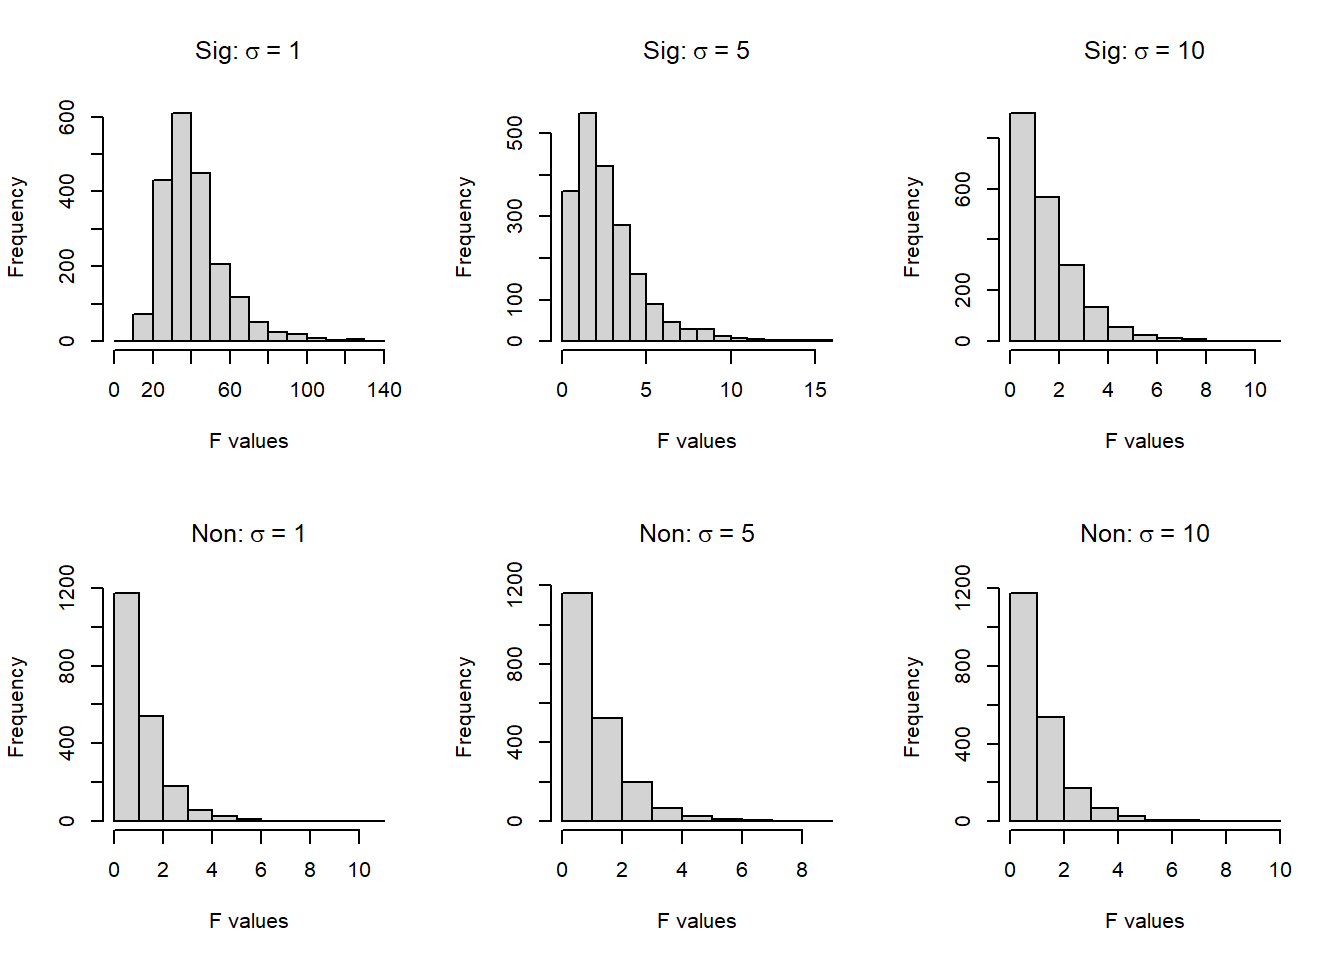
\includegraphics{week_1_quiz_files/figure-latex/unnamed-chunk-4-1.pdf}

The standard deviation of Petal.Length is 1.7652982

\hypertarget{section}{%
\subsection{5.}\label{section}}

\begin{verbatim}
 str(z)

 min(z[[1]])

 max(z[[2]])

 mean(z[[3]])
\end{verbatim}

\hypertarget{where-were-the-measurements-taken-in-the-airquality-dataset}{%
\subsection{6. Where were the measurements taken in the airquality
dataset?}\label{where-were-the-measurements-taken-in-the-airquality-dataset}}

\begin{Shaded}
\begin{Highlighting}[]
\FunctionTok{str}\NormalTok{(airquality)}
\end{Highlighting}
\end{Shaded}

\begin{verbatim}
## 'data.frame':    153 obs. of  6 variables:
##  $ Ozone  : int  41 36 12 18 NA 28 23 19 8 NA ...
##  $ Solar.R: int  190 118 149 313 NA NA 299 99 19 194 ...
##  $ Wind   : num  7.4 8 12.6 11.5 14.3 14.9 8.6 13.8 20.1 8.6 ...
##  $ Temp   : int  67 72 74 62 56 66 65 59 61 69 ...
##  $ Month  : int  5 5 5 5 5 5 5 5 5 5 ...
##  $ Day    : int  1 2 3 4 5 6 7 8 9 10 ...
\end{verbatim}

\begin{Shaded}
\begin{Highlighting}[]
\NormalTok{?airquality}
\end{Highlighting}
\end{Shaded}

\hypertarget{using-the-airquality-dataset-what-is-the-average-wind-speed-in-may}{%
\subsection{7. Using the airquality dataset, what is the average wind
speed in May
?}\label{using-the-airquality-dataset-what-is-the-average-wind-speed-in-may}}

\begin{Shaded}
\begin{Highlighting}[]
\NormalTok{wind\_in\_may }\OtherTok{=}\NormalTok{ airquality}\SpecialCharTok{$}\NormalTok{Wind[airquality}\SpecialCharTok{$}\NormalTok{Month }\SpecialCharTok{==} \DecValTok{5}\NormalTok{]}
\NormalTok{ave\_wind\_in\_may }\OtherTok{=} \FunctionTok{mean}\NormalTok{(wind\_in\_may)}
\end{Highlighting}
\end{Shaded}

The answer is 11.6225806

\hypertarget{using-the-airquality-dataset-what-is-the-average-ozone-measurement-hint-read-the-documentation-of-any-function-that-returns-an-unexpected-result.-you-will-likely-find-a-solution-to-the-issue.}{%
\subsection{8. Using the airquality dataset, what is the average ozone
measurement? Hint: read the documentation of any function that returns
an unexpected result. You will likely find a solution to the
issue.}\label{using-the-airquality-dataset-what-is-the-average-ozone-measurement-hint-read-the-documentation-of-any-function-that-returns-an-unexpected-result.-you-will-likely-find-a-solution-to-the-issue.}}

\begin{Shaded}
\begin{Highlighting}[]
\FunctionTok{mean}\NormalTok{(airquality}\SpecialCharTok{$}\NormalTok{Ozone, }\AttributeTok{na.rm =} \ConstantTok{TRUE}\NormalTok{)}
\end{Highlighting}
\end{Shaded}

\begin{verbatim}
## [1] 42.12931
\end{verbatim}

The answer is 42.1293103

\hypertarget{using-the-airquality-dataset-create-a-scatter-plot-to-compare-windspeed-and-temperature.-based-on-this-plot-you-believe-that}{%
\subsection{9. Using the airquality dataset, create a scatter plot to
compare windspeed and temperature. Based on this plot, you believe
that:}\label{using-the-airquality-dataset-create-a-scatter-plot-to-compare-windspeed-and-temperature.-based-on-this-plot-you-believe-that}}

\begin{Shaded}
\begin{Highlighting}[]
\FunctionTok{plot}\NormalTok{(airquality}\SpecialCharTok{$}\NormalTok{Wind, airquality}\SpecialCharTok{$}\NormalTok{Temp)}
\end{Highlighting}
\end{Shaded}

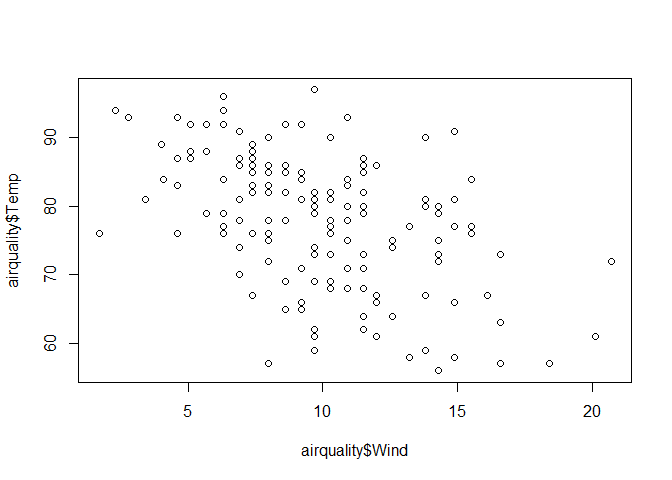
\includegraphics{week_1_quiz_files/figure-latex/unnamed-chunk-8-1.pdf}
There seems to be a weak correlation between wind speed and temperature.
When the temperature increases, the wind speed decreases.

\hypertarget{what-proportion-of-the-elements-of-x-are-larger-than-2-in-magnitude}{%
\subsection{10. What proportion of the elements of x are larger than 2
in
magnitude?}\label{what-proportion-of-the-elements-of-x-are-larger-than-2-in-magnitude}}

\begin{Shaded}
\begin{Highlighting}[]
\FunctionTok{set.seed}\NormalTok{(}\DecValTok{1337}\NormalTok{)}
\NormalTok{x }\OtherTok{=} \FunctionTok{rnorm}\NormalTok{(}\DecValTok{10000}\NormalTok{)}
\NormalTok{index\_larger\_than\_2 }\OtherTok{=}\NormalTok{ x }\SpecialCharTok{\textgreater{}} \DecValTok{2} \SpecialCharTok{|}\NormalTok{ x }\SpecialCharTok{\textless{}} \SpecialCharTok{{-}}\DecValTok{2}
\NormalTok{num\_x\_mag\_larg\_2 }\OtherTok{=} \FunctionTok{length}\NormalTok{(index\_larger\_than\_2[index\_larger\_than\_2 }\SpecialCharTok{==} \ConstantTok{TRUE}\NormalTok{])}
\NormalTok{num\_x\_mag\_larg\_2 }\SpecialCharTok{/} \FunctionTok{length}\NormalTok{(x)}
\end{Highlighting}
\end{Shaded}

\begin{verbatim}
## [1] 0.0444
\end{verbatim}

The answer is 0.0444

\hypertarget{write-a-function-called-f-that-has-a-single-argument-input-with-a-default-value-of-42-which-is-assumed-to-be-a-vector-of-numeric-values.-the-function-should-output-a-vector-that-is-input-but-with-any-negative-values-replaced-with-0.}{%
\subsection{11. Write a function called f that has a single argument
input with a default value of 42 which is assumed to be a vector of
numeric values. The function should output a vector that is input but
with any negative values replaced with
0.}\label{write-a-function-called-f-that-has-a-single-argument-input-with-a-default-value-of-42-which-is-assumed-to-be-a-vector-of-numeric-values.-the-function-should-output-a-vector-that-is-input-but-with-any-negative-values-replaced-with-0.}}

\begin{Shaded}
\begin{Highlighting}[]
\NormalTok{f }\OtherTok{\textless{}{-}} \ControlFlowTok{function}\NormalTok{(}\AttributeTok{input =} \FunctionTok{c}\NormalTok{(}\DecValTok{42}\NormalTok{)) \{}
\NormalTok{  output }\OtherTok{=} \FunctionTok{rep}\NormalTok{(}\DecValTok{0}\NormalTok{, }\FunctionTok{length}\NormalTok{(input)) }\CommentTok{\# initialize output}
  \ControlFlowTok{for}\NormalTok{(index }\ControlFlowTok{in} \DecValTok{1}\SpecialCharTok{:}\FunctionTok{length}\NormalTok{(input))\{}
\NormalTok{    output[index] }\OtherTok{=} \FunctionTok{ifelse}\NormalTok{(input[index] }\SpecialCharTok{\textless{}} \DecValTok{0}\NormalTok{, }\DecValTok{0}\NormalTok{, input[index])}
\NormalTok{  \}}
  \FunctionTok{return}\NormalTok{(output)}
\NormalTok{\}}

\CommentTok{\# a test}
\FunctionTok{f}\NormalTok{(}\FunctionTok{c}\NormalTok{(}\SpecialCharTok{{-}}\DecValTok{1}\NormalTok{, }\DecValTok{2}\NormalTok{, }\SpecialCharTok{{-}}\DecValTok{3}\NormalTok{, }\DecValTok{4}\NormalTok{, }\SpecialCharTok{{-}}\DecValTok{5}\NormalTok{))}
\end{Highlighting}
\end{Shaded}

\begin{verbatim}
## [1] 0 2 0 4 0
\end{verbatim}

\begin{Shaded}
\begin{Highlighting}[]
\CommentTok{\# quiz}
\FunctionTok{set.seed}\NormalTok{(}\DecValTok{42}\NormalTok{)}
\NormalTok{x }\OtherTok{=} \FunctionTok{rnorm}\NormalTok{(}\DecValTok{100}\NormalTok{, }\AttributeTok{mean =} \DecValTok{0}\NormalTok{, }\AttributeTok{sd =} \DecValTok{10}\NormalTok{)}
\FunctionTok{mean}\NormalTok{(}\FunctionTok{f}\NormalTok{(}\AttributeTok{input =}\NormalTok{ x)) }\SpecialCharTok{{-}} \FunctionTok{f}\NormalTok{()}
\end{Highlighting}
\end{Shaded}

\begin{verbatim}
## [1] -37.70725
\end{verbatim}

\hypertarget{create-three-vectors-x0-x1-and-y.-each-should-have-a-length-of-30-and-store-the-following}{%
\subsection{12. Create three vectors x0, x1, and y. Each should have a
length of 30 and store the
following:}\label{create-three-vectors-x0-x1-and-y.-each-should-have-a-length-of-30-and-store-the-following}}

\begin{Shaded}
\begin{Highlighting}[]
\CommentTok{\# create vectors x0 and x1}
\NormalTok{n }\OtherTok{=} \DecValTok{30}

\CommentTok{\# x0: Each element should be the value 1 }
\NormalTok{x0 }\OtherTok{=} \FunctionTok{rep}\NormalTok{(}\DecValTok{1}\NormalTok{, n)}

\CommentTok{\#x1: The first 30 square numbers, starting from 1 (so 1, 4, 9, etc.) }
\NormalTok{x1 }\OtherTok{=}\NormalTok{ (}\DecValTok{1}\SpecialCharTok{:}\NormalTok{n)}\SpecialCharTok{\^{}}\DecValTok{2}

\FunctionTok{set.seed}\NormalTok{(}\DecValTok{42}\NormalTok{)}
\NormalTok{y  }\OtherTok{=} \DecValTok{5} \SpecialCharTok{*}\NormalTok{ x0 }\SpecialCharTok{+}\NormalTok{ x1 }\SpecialCharTok{+} \FunctionTok{rnorm}\NormalTok{(}\AttributeTok{n =} \DecValTok{30}\NormalTok{, }\AttributeTok{mean =} \DecValTok{0}\NormalTok{ , }\AttributeTok{sd =} \DecValTok{1}\NormalTok{)}
\end{Highlighting}
\end{Shaded}

The mean of y is 320.2352535.

\hypertarget{create-a-matrix-x-with-columns-x0-and-x1.-report-the-sum-of-the-elements-in-rows-17-and-19.}{%
\subsection{13. Create a matrix X with columns x0 and x1. Report the sum
of the elements in rows 17 and
19.}\label{create-a-matrix-x-with-columns-x0-and-x1.-report-the-sum-of-the-elements-in-rows-17-and-19.}}

\begin{Shaded}
\begin{Highlighting}[]
\CommentTok{\# x0: Each element should be the value 1 }
\NormalTok{x0 }\OtherTok{=} \FunctionTok{rep}\NormalTok{(}\DecValTok{1}\NormalTok{, n)}

\CommentTok{\#x1: The first 30 square numbers, starting from 1 (so 1, 4, 9, etc.) }
\NormalTok{x1 }\OtherTok{=}\NormalTok{ (}\DecValTok{1}\SpecialCharTok{:}\NormalTok{n)}\SpecialCharTok{\^{}}\DecValTok{2}

\NormalTok{m }\OtherTok{=} \FunctionTok{cbind}\NormalTok{(x0, x1)}
\NormalTok{m[}\DecValTok{17}\NormalTok{,]}
\end{Highlighting}
\end{Shaded}

\begin{verbatim}
##  x0  x1 
##   1 289
\end{verbatim}

\begin{Shaded}
\begin{Highlighting}[]
\NormalTok{m[}\DecValTok{19}\NormalTok{,]}
\end{Highlighting}
\end{Shaded}

\begin{verbatim}
##  x0  x1 
##   1 361
\end{verbatim}

The sum is 652

\hypertarget{use-matrix-operations-to-create-a-new-matrix-beta_hat-defined-as-follows.-report-the-sum-of-the-values-stored-in-this-matrix.}{%
\subsection{14. Use matrix operations to create a new matrix beta\_hat
defined as follows. Report the sum of the values stored in this
matrix.}\label{use-matrix-operations-to-create-a-new-matrix-beta_hat-defined-as-follows.-report-the-sum-of-the-values-stored-in-this-matrix.}}

\(\hat\beta = (X^TX)^{-1}X^Ty\)

\begin{Shaded}
\begin{Highlighting}[]
\CommentTok{\# create vectors x0 and x1}
\NormalTok{n }\OtherTok{=} \DecValTok{30}

\CommentTok{\# x0: Each element should be the value 1 }
\NormalTok{x0 }\OtherTok{=} \FunctionTok{rep}\NormalTok{(}\DecValTok{1}\NormalTok{, n)}

\CommentTok{\#x1: The first 30 square numbers, starting from 1 (so 1, 4, 9, etc.) }
\NormalTok{x1 }\OtherTok{=}\NormalTok{ (}\DecValTok{1}\SpecialCharTok{:}\NormalTok{n)}\SpecialCharTok{\^{}}\DecValTok{2}

\FunctionTok{set.seed}\NormalTok{(}\DecValTok{42}\NormalTok{)}
\NormalTok{y  }\OtherTok{=} \DecValTok{5} \SpecialCharTok{*}\NormalTok{ x0 }\SpecialCharTok{+}\NormalTok{ x1 }\SpecialCharTok{+} \FunctionTok{rnorm}\NormalTok{(}\AttributeTok{n =} \DecValTok{30}\NormalTok{, }\AttributeTok{mean =} \DecValTok{0}\NormalTok{ , }\AttributeTok{sd =} \DecValTok{1}\NormalTok{)}

\NormalTok{x }\OtherTok{=} \FunctionTok{cbind}\NormalTok{(x0, x1)}

\NormalTok{x\_t }\OtherTok{=} \FunctionTok{t}\NormalTok{(x)}

\NormalTok{beta }\OtherTok{=} \FunctionTok{solve}\NormalTok{(x\_t }\SpecialCharTok{\%*\%}\NormalTok{ x) }\SpecialCharTok{\%*\%}\NormalTok{ (x\_t }\SpecialCharTok{\%*\%}\NormalTok{y)}
\end{Highlighting}
\end{Shaded}

The sum of \(\hat\beta\) is 6.4278989

\hypertarget{perform-and-report-the-result-of-the-following-operation}{%
\subsection{15. Perform and report the result of the following
operation}\label{perform-and-report-the-result-of-the-following-operation}}

\(\hat y = X\hat\beta\)

\(\sum_{i=1}^{30}(y_i - \hat y_i)^2\)

\begin{Shaded}
\begin{Highlighting}[]
\NormalTok{y\_hat }\OtherTok{=}\NormalTok{ x }\SpecialCharTok{\%*\%}\NormalTok{ beta}
\NormalTok{result }\OtherTok{=} \FunctionTok{sum}\NormalTok{((y }\SpecialCharTok{{-}}\NormalTok{ y\_hat)}\SpecialCharTok{\^{}}\DecValTok{2}\NormalTok{)}
\end{Highlighting}
\end{Shaded}

The result is 42.6769814

\end{document}
